
\begin{frame}
    \frametitle{Steady state probabilities - Custom network}
    \centering

    \tiny
    \begin{equation*}
        Q = 
        \begin{blockarray}{cccccccc}
            (0, 0) & (0, 1) & (0, 2) & & (2, 3) & (2, 4) & &\\
            & & & & & & & &\\
            \begin{block}{(cccccc)cc}
                -\lambda_1 - \lambda_2 & \lambda_1 + \lambda_2 & 0 & \dots & 0 & 0 & & (0,0) \\
                \mu & -\mu - \lambda_1 - \lambda_2 & \lambda_1 + \lambda_2 & \dots & 0 & 0 & & (0,1) \\
                0 & 2\mu & -2\mu - \lambda_1 - \lambda_2 & \dots & 0 & 0 & & (0,2) \\
                \vdots & \vdots & \vdots & \ddots & \vdots & \vdots \\
                0 & 0 & 0 & \dots & -\lambda_1 - 3\mu & \lambda_1 & & (2,3) \\
                0 & 0 & 0 & \dots & 3\mu & -3\mu & & (2,4) \\
            \end{block}
        \end{blockarray}    
    \end{equation*}
    \normalsize

    \begin{multicols}{2}
        \begin{tikzpicture}[-, node distance = 0.6cm, auto, every node/.style={scale=0.45}]
            \node[state] (one) {(0,0)};
            \node[state, right=of one] (two) {(0,1)};
            \node[state, right=of two] (three) {(0,2)};
            \node[state, right=of three] (four) {(0,3)};
            \node[state, right=of four] (five) {(0,4)};
            \node[state, below=of three] (three_one) {(1,2)};
            \node[state, below=of three_one] (three_two) {(2,2)};
            \node[state, below=of four] (four_one) {(1,3)};
            \node[state, below=of four_one] (four_two) {(2,3)};
            \node[state, below=of five] (five_one) {(1,4)};
            \node[state, below=of five_one] (five_two) {(2,4)};
            \draw[every loop]
                (one) edge[bend left] node {\( \lambda_1 + \lambda_2 \)} (two)
                (two) edge[bend left] node {\( \mu \)} (one)
                (two) edge[bend left] node {\( \lambda_1 + \lambda_2 \)} (three)
                (three) edge[bend left] node {\( 2\mu \)} (two)
                (three) edge[bend left] node {\( \lambda_1 \)} (four)
                (four) edge[bend left] node {\( 3\mu \)} (three)
                (four) edge[bend left] node {\( \lambda_1 \)} (five)
                (five) edge[bend left] node {\( 3\mu \)} (four)
                (three) edge[bend left] node {\( \lambda_2 \)} (three_one)
                (three_one) edge[bend left] node {\( 2\mu \)} (three)
                (three_one) edge[bend left] node {\( \lambda_1 \)} (four_one)
                (four_one) edge[bend left] node {\( 3\mu \)} (three_one)
                (four_one) edge[bend left] node {\( \lambda_1 \)} (five_one)
                (five_one) edge[bend left] node {\( 3\mu \)} (four_one)
                (four) edge node {\( \lambda_2 \)} (four_one)
                (five) edge node {\( \lambda_2 \)} (five_one)
                (three_one) edge[bend left] node {\( \lambda_2 \)} (three_two)
                (three_two) edge[bend left] node {\( 2\mu \)} (three_one)
                (four_one) edge node {\( \lambda_2 \)} (four_two)
                (five_one) edge node {\( \lambda_2 \)} (five_two)
                (three_two) edge[bend left] node {\( \lambda_1 \)} (four_two)
                (four_two) edge[bend left] node {\( 3\mu \)} (three_two)
                (four_two) edge[bend left] node {\( \lambda_1 \)} (five_two)
                (five_two) edge[bend left] node {\( 3\mu \)} (four_two)
                ;
        \end{tikzpicture}
        \columnbreak

        \tiny
        \vspace*{-0.9cm}
        \begin{equation*}
            \frac{d \pi}{dt} = \pi Q = 0, \qquad \sum \pi_{(u,v)} = 1
        \end{equation*}
        \begin{equation*}
            \pi =
            \begin{bmatrix}
                \pi_{(0,0)} \\
                \pi_{(0,1)} \\
                \pi_{(0,2)} \\
                \vdots \\
                \pi_{(2,3)} \\
                \pi_{(2,4)} \\
            \end{bmatrix} 
        \end{equation*}
        \columnbreak
    \end{multicols}

\end{frame}



\begin{frame}
    \frametitle{Steady state probabilities - Comparison}

    \centering
    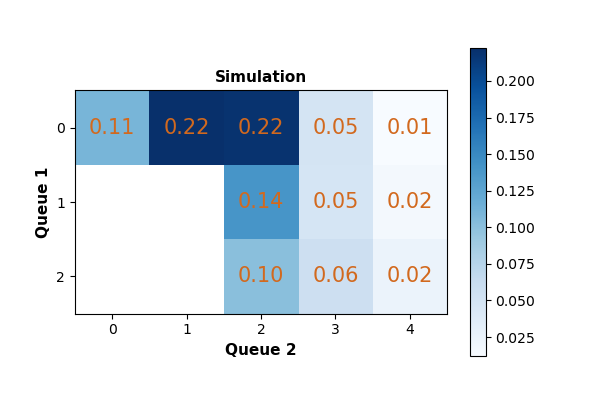
\includegraphics[scale=0.35]{Bin/state_probs_comparison/simulation.png}
    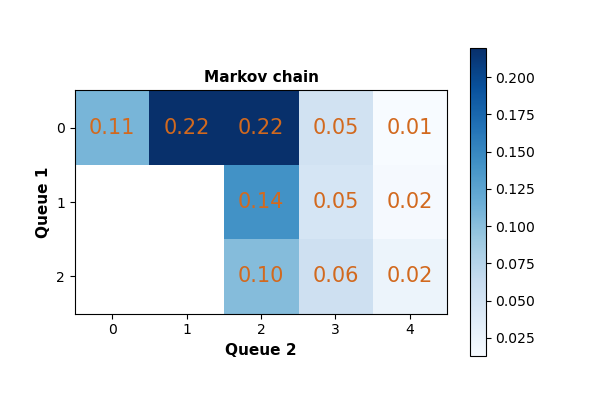
\includegraphics[scale=0.35]{Bin/state_probs_comparison/markov.png}
    
    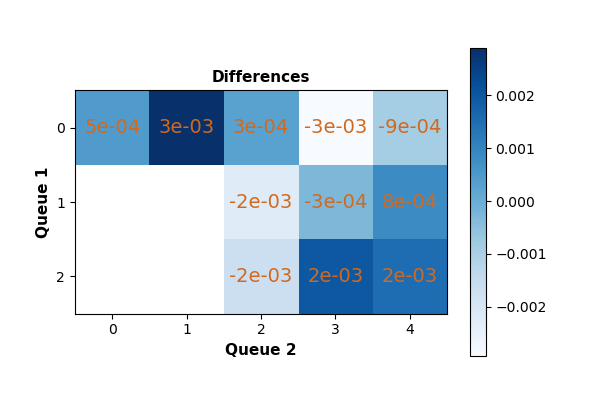
\includegraphics[scale=0.4]{Bin/state_probs_comparison/diff.png}

\end{frame}
